% BACKGROUND & RELATED WORK
%
% !TEX root = ../thesis-main.tex
%
\chapter{Background and related work}
\label{chap:background}

%\cleanchapterquote{You can’t do better design with a computer, but you can speed up your work enormously.}{Wim Crouwel}{(Graphic designer and typographer)}


	\section{Pronunciation in foreign language education}
	\label{sec:bkgd:l2ed}
%	
%	The difficulties posed by including pronunciation in the foreign language classroom curriculum will be discussed in this section, leading to the conclusion that CAPT can help make pronunciation training more accessible by overcoming some of these difficulties (e.g. teacher-to-student ratio). Relevant findings from a variety of works on pronunciation teaching in the classroom will be presented .

%\citep{Derwing2005,Dlaska2013,Hirschfeld2007,Mehlhorn2005}

In the foreign language classroom, and the German language classroom in particular, less focus has traditionally been placed on pronunciation than other aspects of language education, such as grammar and vocabulary %; %\citep{Neri2002,Derwing2005}. 
%this is particularly true for German 
\citep{Hirschfeld2007}.
However, even when pronunciation is taught in the classroom, a number of factors may limit the effectiveness of that training. %\citep{Neri2002,Derwing2005}. 
First of all, partly thanks to a historical lack of communication between the fields of speech science and foreign language education, many teachers lack the training in phonetics and phonology to provide helpful feedback to students and correct their articulation \citep{Derwing2005,Hirschfeld2007}. Secondly, high student-to-teacher ratios may prevent teachers from giving adequate attention and feedback to individual students, and limit the amount of time each student can practice speaking \citep{Neri2002}. Furthermore, anxiety about speaking the L2 in front of their peers may make students less willing to practice speaking, and less able to absorb corrective feedback \citep{Neri2002}. 
%\TODO{individual/specific citations for each point above? Hirschfeld?}



%Fortunately, recent years have seen a growing interest in sound pronunciation pedagogy in the FLE community 

Although much work still needs to be done to improve our understanding of how best to teach pronunciation, existing research reveals a few general considerations that must be kept in mind.
	First of all, it is important to note that 
intelligibility, and not lack of a ``foreign accent,'' is generally considered to be the most important goal of pronunciation training \citep{Munro1999,Neri2002,Derwing2005,Field2005,Witt2012}. %\TODO{\citep{Hahn2004}?}
As \textcite{Field2005} and others point out, the exact definition of the term \textit{intelligibility} is a topic of debate in the literature, as is the question of whether and how it differs from the notion of comprehensibility; 
here, let us follow \textcite[p.~289]{Munro1999} in understanding intelligibility broadly as ``the extent to which a speaker’s message is actually understood by a listener.'' 
%here, intelligibility is understood broadly as the degree to which the \TODO{content} of the (L2) speaker's utterance is made clear to the listener.
	

Research on the impact of various types of pronunciation errors on intelligibility tends to indicate that errors on the prosodic (suprasegmental) level may hinder intelligibility more than segmental errors.
%
\TODO{\textit{transitions in this paragraph}}
% 
In a study of nonnative English speakers from various native language (L1) backgrounds, \textcite{Anderson-Hsieh1992} found that overall pronunciation ratings, which reflect intelligibility, correlated more strongly with measures of prosodic accuracy than with accuracy with respect to segmental sounds or syllable structure.
%
Research by \textcite{Hahn2004} points to the particular importance of primary sentence stress, e.g. the accentuation of new or contrasting words in a given sentence, to the intelligibility of L2 English speakers, especially with respect to the way in which these speakers (fail to) use intonation to convey stress.
%
%\TODO{\citep{Derwing2005}}
%
%\TODO{lexical stress errors have been found to impact intelligibility when the L2 is German is the L2 \citep{Hirschfeld1994,Hirschfeld2007}}
Though there exists relatively little research on the impact of various pronunciation errors on intelligibility in German specifically, some studies suggest that prosodic errors, and lexical stress errors especially, may hinder intelligibility of L2 speech more than other types of errors \citep{Hirschfeld1994,Hirschfeld2007}.



To reduce these and other types of errors in learner speech,
%training (e.g. in the form of listening exercises) which helps 
listening exercises designed to help 
learners perceive differences between correct and erroneous pronunciations
%has 
have been found to be valuable, with some work suggesting that perception training can have a positive impact on the intelligibility of L2 speech, even in the absence of exercises or feedback concerned with production \citep{Derwing2005,Hirschfeld2007}}.
%
However, 
%some researchers stress 
other research suggests that production-oriented training with corrective feedback on pronunciation errors produces bigger performance gains. %\citep{Dlaska2013}. 
%\TODO{expand}
%
%\TODO{transition} he importance of individualized corrective feedback is also generally acknowledged.
%\citep{Neri2002,Mehlhorn2005,Dlaska2013}, 
%
%\TODO{\citep{Neri2002}}
As \textcite{Neri2002} point out, corrective feedback from human instructors has been shown to help adult L2 learners notice errors in their pronunciation more than implicit feedback in the form of exposure to speech from L1 speakers of the target language, enabling them to start working towards correcting these errors and thus improving their pronunciation.
This supports the claims of \textcite{Mehlhorn2005} regarding the importance of individualized pronunciation coaching as a way to help L2 German learners become more cognizant of their pronunciation deviations as they take autonomous control of their own pronunciation learning.
%
%\TODO{corrective fb more important than perception training (or stg?) \citep{Dlaska2013}} \TODO{Explicit FB is necessary; learners have trouble identifying their errors when simply asked to listen to what they said \citep{Dlaska2013}}
In a study of L2 German speakers from a variety of L1 backgrounds, \textcite{Dlaska2013} compared the effects of implicit and explicit feedback on the improvement in comprehensibility of the L2 learners' speech, and found that individualized, explicit, corrective feedback from a human language instructor led to more substantial improvements in comprehensibility than the implicit feedback of listening to the learner's own recorded utterance or that of a model native speaker; their findings seem to point to the difficulties learners may have in identifying their own errors, and confirm the importance of offering explicit feedback in L2 pronunciation instruction. 
%

It is thus generally evident that individualized corrective feedback is quite important for L2 pronunciation learning, including L2 German learning specifically; however, there remains much to be learned about exactly when and how feedback can be most effective. This is the motivation behind the 
%feedback generation module of the proposed tool 
diversity of feedback types implemented in the \TODO{de-stress} 
%Computer-Assisted Pronunciation Training (CAPT) 
system (see \cref{chap:feedback}); as described in the previous chapter, this system is intended to facilitate finer-grained research on the effects of such feedback on the acquisition of L2 German word prosody by L1 French speakers.







\section{Computer-Assisted Pronunciation Training}
\label{sec:bkgd:capt}

\TODO{REORGANIZE THIS SECTION}

In recent decades, the educational value of speech technologies has been well demonstrated \citep{Eskenazi2009}, with 
Computer-Assisted Pronunciation Training%
\footnote{Also known as Computer-Assisted Pronunciation Teaching or Tutoring} (CAPT) 
emerging as one important educational application for foreign-language education (FLE) \citep{Neri2002,Delmonte2011,Witt2012}. 
%Computer-Assisted Pronunciation Training\footnote{Also known as Computer-Assisted Pronunciation Teaching or Tutoring} (CAPT) stands to help make pronunciation training more accessible by overcoming some of these difficulties. 
With CAPT, student-to-teacher ratio is not an issue, as the learner always has the full attention of the digital tutor, and provided an effective curriculum design, a CAPT system can offer learners practically limitless practice opportunities. Interacting with a computer program may also be perceived by the learner as a lower-stakes, more comfortable environment than the classroom, where they may feel too intimidated to practice speaking in the L2 \citep{Neri2002}. But perhaps most compelling is the potential for CAPT 
to deliver the type of individualized instruction
%guided by sound science and pedagogy 
which many learners may not otherwise have access to in the L2 classroom, for reasons such as those mentioned in \cref{sec:bkgd:l2ed}.
%Much of the recent interest in CAPT stems from its potential to deliver the type of individualized pronunciation instruction, guided by sound science and pedagogy, which many learners may not have access to in the classroom, as just discussed.
%
%Indeed, in recent decades, the educational value of speech technologies has been well demonstrated \citep{Eskenazi2009}, with CAPT emerging as one important educational application for foreign-language education (FLE) \citep{Neri2002,Delmonte2011,Witt2012}. 
%	%CAPT is attractive from the pedagogical perspective, as its potential to deliver individualized, extended practice poises it to overcome some of the hurdles of teacher-led pronunciation training described in \cref{sec:bkgd:l2ed} below \citep{Neri2002,Derwing2005}. 
However, as \textcite{Derwing2005} point out, for CAPT to be effective, it must be informed by research on not only speech technology, but both speech production and perception on the one hand, and language acquisition and pedagogy on the other.
With this in mind, an overarching aim of this thesis is to take initial steps toward the development of German CAPT technology which takes into account information from these diverse fields. 
%	This section places CAPT in the context of foreign-language pronunciation instruction (\cref{sec:bkgd:l2ed}), and describes a few recent CAPT systems which incorporate training in prosody (\cref{sec:capt:systems}). \TODO{why prosody?}
%
%	
%
%
%	\subsection{Computer-based and intelligent tutoring systems?} 
%	\label{sec:capt:its}
%	%TODO is this section necessary?
%	
%	This section would serve as a domain-independent overview of CBT and ITS, and the advantages such systems can bring when deployed in schools or used individually.
%	
   % \subsection{Prosody in existing CAPT systems}
	\label{sec:capt:systems}
		
	The viability of CAPT has been demonstrated by a variety of systems and tools that have been developed in both academic and commercial contexts. Some focus on overall assessment of pronunciation or fluency, and others on the detection and correction of individual pronunciation errors \citep{Eskenazi2009}; the tool developed in this work falls into the latter category. In error-focused systems, a distinction has typically been drawn between phonemic errors, e.g. the substitution, insertion, or deletion of a segmental speech sound, and prosodic errors, such as those related to stress/accent, intonation, or rhythm \citep{Witt2012}. As discussed in the previous section, word-prosodic errors may have a larger impact on intelligibility than segmental errors, and are therefore the focus of this work (see \cref{sec:bkgd:targeting} below). 
	\TODO{\textit{rewrite} With this in mind, a few prosody-aware CAPT systems relevant to this thesis are discussed below; comprehensive overviews and comparisons of these and many other systems are given by \textcite{Neri2002,Eskenazi2009,Delmonte2011,Witt2012}.  }
	
	%\subsubsection{Automatic processing of learner speech}
	\subsection{Automatic processing of learner speech}
		
	Both the diagnosis and feedback modules of the CAPT tool developed in this work build to a great extent on previous work by researchers in the speech group at LORIA\footnote{\url{http://www.loria.fr/}} in Nancy, France, many of whom are also involved in the IFCASL project (see \cref{sec:intro:ifcasl}). 
	%
	% \TODO{\textit{This part about segmentation doesn't really fit in with the prosody-in-CAPT discussion - find a better place for it.}}
	 Their work has, on the one hand, investigated the task of automatically recognizing and segmenting learners' speech, and determining how this possibly incorrect automatic segmentation can be effectively utilized in the context of pronunciation tutoring, particularly at the prosodic level \citep{Mesbahi2011,Orosanu2012}; 
	%TODO {see \cref{chap:diagnosis} for a discussion of how this thesis will build upon that work. \textit{Details \& de-proposal-ize}}
	
	%\sub
	\subsection{The \textit{Snorri} suite and \textit{Jsnoori}}
	\label{sec:capt:snoori}
	
	%Additionally, the group has developed
	Another important contribution of the LORIA group is 
	the \textit{Snorri/Snoori} suite of software, 
	which includes the now-outdated original \textit{Snorri} developed in 1987 \citep{Fohr1989} and the Unix adaptation thereof developed shortly thereafter,
	a later Windows port, \textit{WinSnorri} \citep{Laprie1999},
	%and its partial Java port, Jsnoori {Parole2013}, 
	and most recently a partial Java port of WinSnorri, \textit{Jsnoori}\footnote{\url{http://jsnoori.loria.fr}} \citep{Parole2013}, which is still under active development, and is the version of the \textit{Snorri} suite most relevant to this work.
	
	\TODO{summary of speech processing capabilities of the Snooris \citep{Fohr1989,Laprie1999}}
	%, without mention of application to L2 acquisition. Then...}
	
	Though the \textit{Snorri} programs were originally developed primarily as research tools for speech scientists %\TODO{\textit{necessary to cite again so soon?} 
	\citep{Fohr1989,Laprie1999}, 
	the utility of such software
	%, and especially of resynthesized feedback, 
	for pronunciation teaching has been explored by the LORIA team \citep{Bonneau2004,Henry2007,Bonneau2011},
	% \citeauthor{Bonneau2004} (\citeyear{Bonneau2004,Bonneau2011}) \TODO{add \citep{Henry2007}},
	% \textcite{Bonneau2011}, 
	who have used 
	%\TODO{\textit{correct?} WinSnoori} 
	this software to assess and deliver feedback on lexical stress in L1 French speakers' pronunciation of English words. 
	%
	%\TODO{transition}
In its role as a CAPT tool, Jsnoori 
takes as input a learner utterance, a native reference utterance, and segmentations of each, perform an acoustic comparison of the two utterances, and deliver feedback on the learner's speech in the form of e.g. annotated displays of the speech signal and spectrogram of each. Moreover, auditory feedback can be delivered 
%thanks to the capability of 
by
resynthesizing the learner's utterance to match the pitch contour and timing of the reference, without modifying the voice quality of the utterance, such that the learner can hear the ``correct'' pronunciation in their own voice. 
%
	\TODO{more details about those papers} 
	
	
	\TODO{Jsnoori screenshot}
	

As described in \cref{chap:diagnosis,chap:feedback}, 
the Jsnoori software is vital to this thesis project;
the prototype CAPT tool developed in this work 
utilizes the signal processing capabilities of Jsnoori 
%and
%builds on the error diagnosis functionality of Jsnoori 
for speech analysis and error diagnosis (see \cref{chap:diagnosis}), 
and leverages its feedback generation capabilities to deliver  a more diverse, and potentially more effective, range of feedback types (see \cref{chap:feedback}). 
	
	% \citep{Bonneau2011,Fohr1996,Fohr2012,Mesbahi2011,Orosanu2012}. The Jsnoori/WinSnoori software \citep{Parole2013}
%which this group has developed will be instrumental in the construction of the CAPT tool. 

	%\sub
	\subsection{The \textit{Fluency} pronunciation trainer}
	\label{sec:capt:fluency}
	
	This work also draws from research on two systems developed at Carnegie Mellon University.
%, namely the Fluency pronunciation trainer
%\citep{%
%	%Eskenazi1998,%
%	Eskenazi2000,%
%	%Probst2002%
%	} 
%and the Project LISTEN Reading Tutor \citep{%
%	%Mostow1999,	
%	%Duong2011,
%	%Sitaram2011,
%	Mostow2012,
%	%Weber2010
%	}. 
%
	The first of these, the Fluency pronunciation trainer \citep{Eskenazi1998,Eskenazi2000}, is a CAPT system placing particular emphasis on
%prosody and 
user-adaptivity, corrective articulatory feedback, and the integration of perceptual training (e.g. listening exercises). As with the work at LORIA described above, the Fluency system evaluates learners' speech via comparison with that of a native reference speaker, and \textcite{Probst2002} found that selecting a ``golden speaker'' whose voice closely matched the learner's improved learning gains. 
%TODO {more about golden speaker?} 
Fluency also implements an error-catching step to reject utterances which do not match the expected text \citep{Eskenazi2000}, in the same vein as that of \textcite{Mesbahi2011,Orosanu2012}. \textcite{Eskenazi2007} report that Fluency's commercial spin-off, NativeAccent\textsuperscript{TM}, has been shown to help real-world users significantly improve their pronunciation skills.
	%In an early version of Fluency, an utterance is elicited from the learner using a targeted question, constraining the learner's response such that a speech recognizer can perform forced alignment on the utterance, while at the same time giving the learner the impression that they have decided what to say (as opposed to simply reading a given sentence out loud).
	
	%\sub
	\subsection{The Project LISTEN Reading Tutor}
	\label{sec:capt:listen}
	
	A second CMU system, the Project LISTEN Reading Tutor \citep{Mostow2012} 
may not strictly be a CAPT tool, as it 
is designed to help children develop reading fluency in their native language. 
However, as 
%To that end, 
it analyzes the prosody of children's read speech to measure reading fluency, and offers feedback on this prosody, 
it is nevertheless very relevant to CAPT and thus this thesis. 
	Indeed, the potential for such a tool, and its underlying technologies, to enhance foreign-language education has already been demonstrated by 
	\textcite{Weber2010}, who deployed the Reading Tutor in English as a second language classes in India with encouraging initial results \TODO{more?}. 
	In the Reading Tutor, the child's read speech is automatically segmented and compared either to a reference utterance by an adult reader, analogous to the native speaker reference in many CAPT systems, or to a generalized model of adult prosody; \textcite{Duong2011} report better performance using the generalized model. Analysis of the pitch and intensity contours of the utterance(s), as well as the duration of words/syllables and the pauses between them, results in an assessment of the child's overall fluency as well as identification of words which have been pronounced (in)correctly, and feedback is delivered visually in real time by revealing the text of each word as it is spoken, with properties such as the position, color, and font size of each word reflecting various aspects of the reader's prosody \citep{Sitaram2011}. Ideas and techniques from the Reading Tutor have influenced both the diagnosis (see \cref{chap:diagnosis}) and feedback (see \cref{chap:feedback}) modules of the proposed CAPT tool. 
	\TODO{which ideas, influenced how?}
	
	\subsection{German and language-independent CAPT}
	\label{sec:capt:german}
	%\TODO{flesh out this paragraph - rephrase subsection heading?}
	The vast majority of CAPT systems which analyze learners' speech at the prosodic level have been developed with English as the target L2, and relatively little work has been done on German.
	%Notable exceptions include
	%\TODO{Delmonte's SLIM?}, 
	In a notable exception particularly relevant to this thesis, 
\citeauthor{Bissiri2006} 
(\citeyear{%
%\citep{%
Bissiri2006,Bissiri2009%
})
 found that L1 Italian speakers' realizations of lexical stress in German improved when they were allowed to listen to 
prosodically-modified recordings of their own speech and that of native speakers (see \TODO{\cref{sec:fb:auditory}}).
%their own utterance resynthesized to reflect the prosody of a reference utterance by a native speaker, as well as when they could listen to an utterance by a native speaker that had been prosodically modified to place 
%prosodically-modified auditory feedback useful for improving L1 Italian speakers' realizations of lexical stress in German \TODO{What did they find out?}.
%
	\citeauthor{Jilka1998}'s (\citeyear{Jilka1998}) use of F0 contour manipulation in studying L1 English speakers' production of German represents another exploration of speech technology applications for German instruction. \TODO{details}
%TODO replace?
%	Ville, for L2 Swedish instruction \citep{Wik2009}, incorporates both perception and production exercises for lexical stress and other prosodic errors, and features an animated virtual character as the tutor.
%

	Language-independent tools have also been developed for teaching prosody, such as WinPitch LTL \citep{Martin2004}, which enables speech signal visualization of prosodic features such as pitch contours as well as manipulation of prosody and comparison to reference utterances, with the intent that a human instructor will guide the learner in using the software and interpreting the visualizations.
	%\TODO{anything else?}
	
	%Other systems mentioned by \textcite{Eskenazi2009,Delmonte2011,Witt2012} may also be briefly described, including tools developed at KTH \citep{Hincks2002,Hincks2009} to teach English prosody.
	
	\TODO{need an outro for this (sub)section?}
	
	
% Alternative organization:
 \section{Lexical stress}
 \label{sec:bkgd:stress}
		%TODO check this section for inaccuracies
		When there is a typological difference between some segmental or prosodic feature(s) of a language learner's L1 compared to the target L2, there is a particular need for pronunciation training to bridge this gap. In the case of the French-German language pair, the prosodic realization of lexical stress is one feature which marks a striking difference between the languages.
		
			In the broadest terms, lexical stress is the phenomenon of how syllables are accentuated within a word  \citep{Cutler2005}. To say that a given syllable in a word is stressed is, generally speaking, to say that that syllable is somehow accorded a more prominent role in the word than other syllables, i.e. that this syllable is perceived as somehow ``standing out'' \citep{Dogil1999}.
			%\TODO{Elaborate} 
			The perceived prominence of a syllable in a word is a function not merely of the segmental characteristics of the uttered syllable, i.e. the speech sounds it contains, but rather of its (relative) suprasegmental properties, namely: %TODO need citation here?
			\begin{itemize}
			\item duration, which equates on the perceptual level to length; %timing;
			\item fundamental frequency (F0), which corresponds to perceived pitch; and
			\item intensity (energy or amplitude), which perceptually equates to loudness.
			\end{itemize}

%TODO more text here? or move text from German vs French section here?
	\subsection{German}
	\label{sec:stress:german}
	
		
		%\subsection{German vs. French}
		%\label{sec:stress:GvF}
		
					As \textcite{Cutler2005} points out, different languages make use of this suprasegmental information in different ways.
			In what are termed free- or variable-stress languages, such as German, Spanish, and English, it is not always possible to predict which syllable in a word will carry the stress, and therefore knowing a word requires, in part, knowing its stress pattern. This allows lexical stress to serve a contrastive function in these languages, such that two words may share exactly the same sequence of phones and nevertheless be distinguished exclusively by their stress pattern, as is the case with \textit{UMfahren} (to drive around) and \textit{umFAHRen} (to run over with a car) in German. %TODO better example of minimal pair
Because stress carries meaning thus, native speakers of such languages are sensitive to stress patterns, and readily able to perceive differences in stress. %TODO wording?
Furthermore, in German, misplaced stress has been shown to disrupt understanding of a word or utterance even in cases where there is no stress-based minimal pair \citep{Hirschfeld1994}, supporting the theory that speakers of free-stress languages rely to a large extent on stress information in the recognition of spoken words \citep{Cutler2005}.

	\subsection{French}
	\label{sec:stress:french}

			However, in the so-called fixed-stress languages, stress is completely predictable, as it always falls on a certain position in the word;
%in French, for example, stress is fixed on the word-final syllable, while 
in Czech and Hungarian, stress always falls on the initial syllable. Lexical stress may not be as crucial to the knowledge of a word in these languages as in the free-stress languages. Furthermore, although lexical stress is realized in these languages, the distinction between stressed and unstressed syllables may be weaker than in free-stress languages.
%
 While many theorists place French 
 %has often been placed 
 into this category of fixed-stress languages, pointing to the fact that word-final syllables are always most prominent when a word is pronounced in isolation,
 %although 
 others argue that
 it may be more properly considered a language without lexical stress, insofar as there is no systematic way in which speakers distinguish a certain syllable from others in the word, aside from the fact that French exhibits phrasal accent, expressed as a lengthening of the final syllable in each prosodic group or phrase \citep{Dupoux2008,Michaux2013}.  
 %
 Regardless, stress at the word level does not serve any contrastive function in French \citep[p.~89]{Michaux2013}, which constitutes a significant difference between this language and a language with variable, contrastive lexical stress such as German or English.
 
% 		\TODO{``French does not have contrastive stress: the standard final prominence in isolated words disappears when they are located in non-final position in a larger word group, leaving a word-group final accent... Rather than being contrastive, this `primary' accent has a demarcative function. \citep[p.~89]{Michaux2013}}
			
		\subsection{Expected pronunciation errors}
		\label{sec:stress:expected}
		As a result of this difference in the sound systems of the two languages,
		native speakers of French may generally be expected to lack the sensitivity to stress patterns possessed by native speakers of German. Indeed, this has been borne out by research by \textcite{Dupoux2008},
		%\citep{Dupoux2001,Dupoux2008},
  who found that native French speakers are ``deaf'' to differences in stress patterns, such that they have great difficulty \TODO{\textit{JT comments} discriminating} between Spanish words which contrast only at the level of stress. This difficulty should also exist for French speakers when they are presented with German words in which the stress pattern is crucial to the word's meaning, as in the minimal pair above. 
  
  In addition to these difficulties with lexical stress perception, French learners of variable-stress languages such as English, German and Dutch have also been shown to have difficulties in producing stress patterns correctly. Research by \citeauthor{Michaux2012} et al. (\citeyear{Michaux2012,Michaux2013}) revealed that, as might be expected given the tendency for word- and/or phrase-final syllable prominence in French just discussed, French learners of Dutch  showed a tendency to stress the final syllables of Dutch words, even when not called for by the canonical stress pattern. \TODO{mention no-stress pattern? happens in English sentence stress with speakers of different L1s \citep{Hahn2004}} 
  Indeed, with regard to German specifically, \textcite{Hirschfeld2007} report that lexical stress is a commonly observed error among L2 speakers with French as L1.
  
% While little research exists specifically investigating the errors of French, 
 In short, based on prior work on French learners of variable-stress languages,
 it can reasonably be expected that L1 French learners of German as L2 will face challenges with both the perception and production of lexical stress, and that the (lack of) lexical stress system in their native language will have an influence on their realization of lexical stress patterns in German words.

		
		
 \section{Targeting lexical stress errors in CAPT}
 \label{sec:bkgd:targeting}
 	Learners of a foreign language typically make a wide variety of pronunciation errors, at both the segmental level (e.g. errors in producing certain vowels or consonants of the target language) and the prosodic level (e.g. errors in the speaker's intonation contour or the duration of certain syllables or words). 
 As it is not feasible to address all of these in a prototype CAPT tool, 
one of the first aims of this work is to identify a single type of error which is well suited to being addressed via CAPT for L1 French/L2 German.
	
	To guide this selection, \TODO{we may consider} 
a set of three criteria that such an error must meet; similar criteria are proposed by \textcite{Neri2002,Cucchiarini2009}.
%The criteria are:
%
%\begin{enumerate}
%\item T
\TODO{reorder to match sections}
First, 
the error must be \textit{produced relatively frequently} by French L1 speakers in their production of L2 German, as it would be a misuse of resources to design a system addressing an error seldom made by learners. %\citep{Neri2002}.
%\item T
Second,
the error must have a significant \textit{impact on the perceived intelligibility} of the learner's speech; 
as the ultimate goal of the system is to help learners communicate more effectively in the L2,
 an error which is commonly made but nevertheless does not impede understanding of the learner's L2 speech, and thus does not hinder communication in the L2, is not an ideal target. 
%\item I
Third,
in order for the CAPT system to provide any meaningful diagnosis and feedback, the error must lend itself to reasonably accurate and reliable  \textit{detection through automatic processing}. 
%
%\end{enumerate}
%
%
As illustrated in \cref{fig:errors}, the best error to target with the CAPT system will fulfill all of these criteria, rather than only one or two of the three. 
	 For example, vowel quality errors (e.g. an L1 French speaker producing a German /\textipa{@}/ as [\textipa{\oe}]) may occur frequently in the L2 speech and may be relatively easy to detect automatically, but may not have a great impact on the intelligibility of the L2 German speech. On the other hand, equally frequent vowel quantity errors (e.g. the L1 French speaker producing a German long /\textipa{a:}/ as [\textipa{a}]) may have a greater impact on intelligibility in some cases, but may be more difficult to reliably identify automatically.

		%\begin{center}
		\begin{figure}[htb]
			\centering
			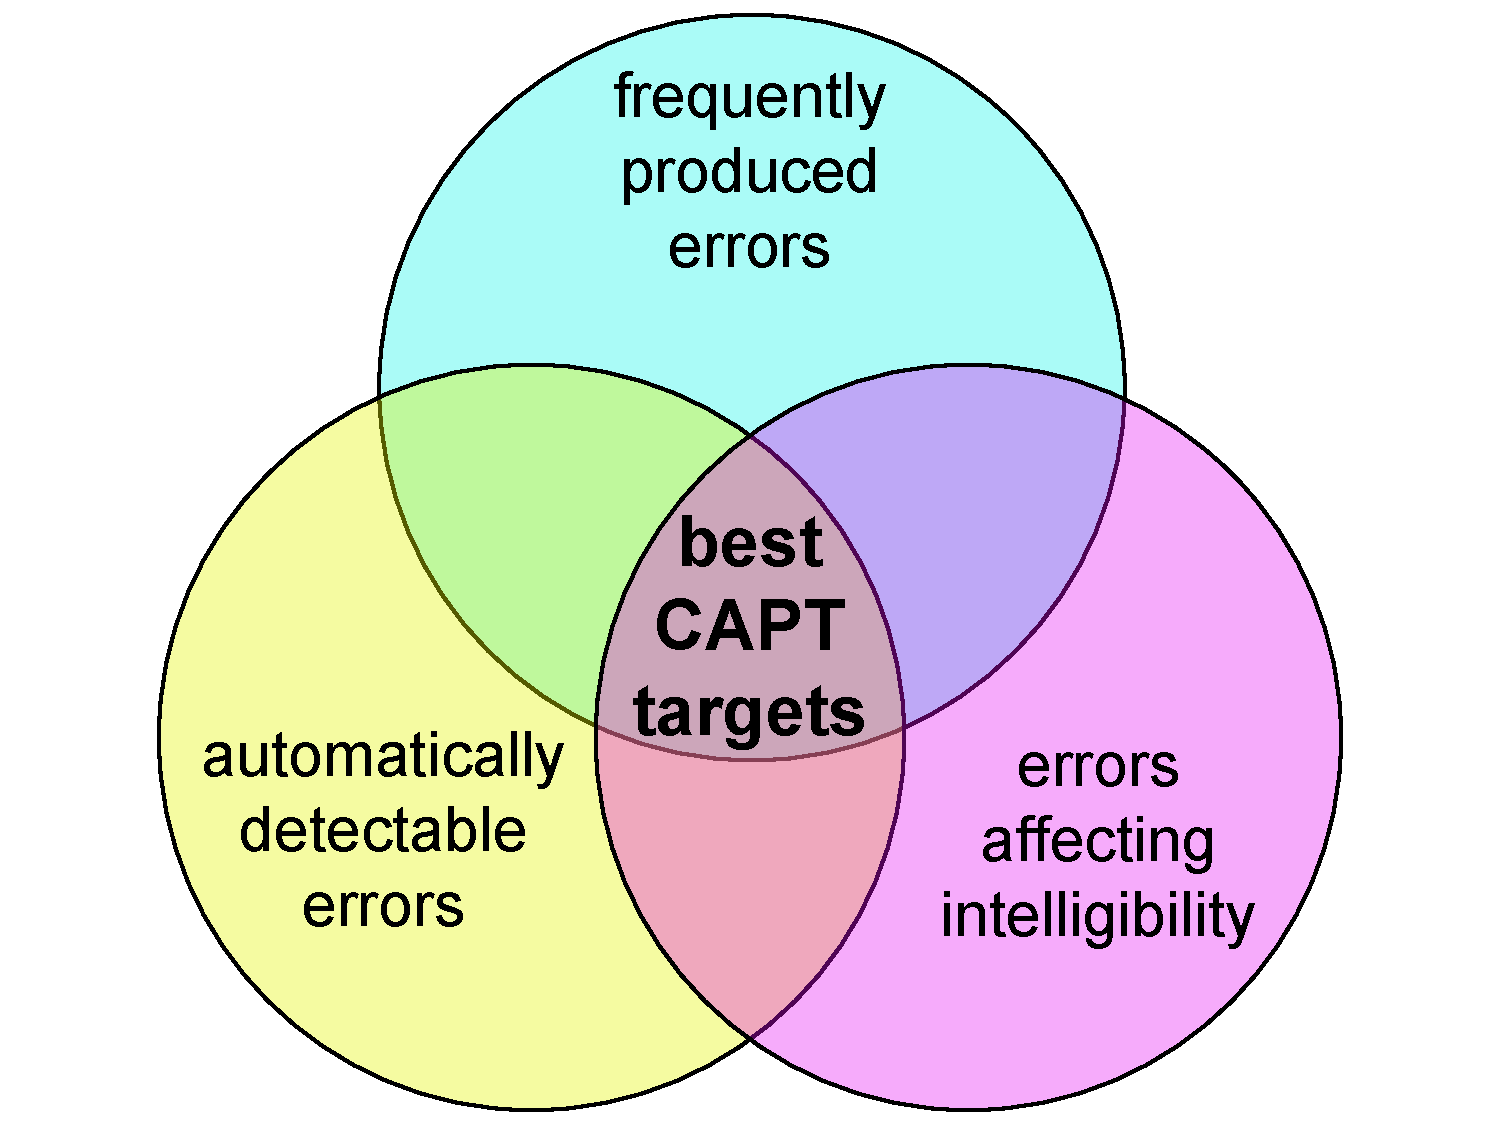
\includegraphics[width=.7\textwidth]{img/error-venn}
			\caption{Criteria for selecting errors to target in a CAPT system.}
			\label{fig:errors}
		\end{figure}
		%\end{center}

	Lexical stress errors 
	%\TODO{e.g.} 
	fulfill all three of these criteria, and this error type has therefore been chosen as the target of the proposed CAPT tool. The remainder of this section 
	%justifies 
	presents the reasoning behind 
	that choice. 
	%This thesis proposes that lexical stress errors are a strong candidate for treatment via CAPT, as this type of error meets all three criteria. 
%	
%	
%
%	 

%
%TODO remove
	%Analysis of the typical and expected errors described in \cref{sec:CAPT4FG:comparison} in terms of these criteria reveals that lexical stress errors are a strong candidate for treatment via CAPT, and will therefore be the focus of the prototype CAPT system described in this thesis. The remainder of this section justifies the selection of this type of error by describing how it fulfills the aforementioned criteria as well or better than any other error type.
%	
%
		\subsection{Impact on intelligibility}
		\label{sec:targeting:intelligibility}
		

	First, as mentioned in \cref{sec:bkgd:l2ed} above, errors related to prosody have 
	often
	%generally
	 been found to have a larger impact on the perceived intelligibility of L2 speakers than segmental errors \citep{Hahn2004,Derwing2005,Witt2012}, and several studies have found lexical stress errors in particular to have in impact on L2 intelligibility
	 % to be particularly important for comprehension 
	 in free-stress languages like English, Dutch, and 
	 %our target language, 
	 German \citep{Hirschfeld1994,Cutler2005,Field2005}.
%Also Swedish \citep{Wik2009}	
	%Research on the impact of various types of pronunciation errors has generally shown that errors related to prosody, and especially to stress, have a larger impact on the perceived intelligibility of the L2 speaker than errors on the segmental level \citep{Derwing2005,Witt2012}. 
	Indeed, studies on perception of German L2 speech have found that among a variety of pronunciation error types, lexical stress errors have one of the most drastic impacts on intelligibility \citep{Hirschfeld1994}.
%
	 %\citep{Warren2009}
	%	
		%Native English speakers are sensitive to lexical stress, among other things\citep{Magen1998}
		%\TODO{recall more content when primary SENTENCE stress is correct \citep{Hahn2004}}
	%	
		Furthermore, lexical stress not only impacts intelligibility on the prosodic level, but may also affect perception of segmental errors in the L2 learner's speech; for example, segmental errors occurring in stressed syllables are more noticeable than those in unstressed syllables \citep{Cutler2005,Michaux2012}. 
	%	
		Additionally, some research indicates that prosodic errors such as lexical stress errors may have more of an impact on perceived foreign accent than segmental errors \citep{Hahn2004,Witt2012}; though it must again be stressed that intelligibility is a more important goal than lack of a foreign accent, insofar as perceived accent may contribute to difficulties being understood by native speakers, this relationship between prosody and accentedness also deserves mentioning.
	% ``Prosody errrors in particular tend to contribute to any perceived accent more so than individual phoneme mispronunciations.'' \citep[p.~6]{Witt2012}
		%		

		\subsection{Frequency of production}
		\label{sec:targeting:frequency}

Secondly, we saw in \cref{sec:bkgd:stress} that perceiving contrasts in lexical stress is notoriously difficult for native French speakers \citep{Cutler2005,Dupoux2008}, and given the strong link between perception and production,
%mentioned earlier (\cref{sec:bkgd:l2ed}), 
this is a good indication that L1 French speakers will regularly make lexical stress errors in an L2 with free, contrastive stress, such as German. \textcite{Bonneau2011} report that in a pilot study of L1 French speakers pronouncing English words, lexical stress was frequently misplaced by beginners; given the similarities of the lexical stress systems of English and German compared to that of French, this is another sign that we can expect such errors to be produced frequently.
%
Indeed, an analysis of lexical stress errors in the IFCASL corpus of non-native (L1 French) German speech conducted as part of this thesis project supports the expectation of frequent lexical stress errors in this particular L1/L2 pair: 
%\TODO{verify/reword if necessary: 
errors were observed at all skill levels, though beginners made many more errors than advanced learners. See \cref{chap:lexstress} for a detailed discussion of these findings.
	

		\subsection{Feasibility of automatic detection}
		\label{sec:targeting:autodetect}

Finally, although much research still needs to be done on automatic detection and diagnosis of lexical stress errors (one of the main motivations behind this work; see \cref{chap:diagnosis}), recent work on this problem has shown encouraging results. As mentioned above, several existing CAPT tools incorporate treatment of lexical stress errors (e.g. \cite{Wik2009,Bonneau2011}), and \textcite{Shahin2012a,Kim2011} have reported success in applying machine learning methods to the classification of lexical stress patterns in English words. 

		%Detecting syllable- or word-level errors may be more feasible than detecting phone-level errors: ``One additional challenge in pronunciation error detection is that a phoneme represents the smallest possible unit compared to the syllable, word, and sentence level. The shorter the unit, the higher will be the variability in the judgment of the pronunciation quality.'' \citep[p.~2]{Witt2012}




	As lexical stress errors thus fulfill the aforementioned criteria for targeting with CAPT, such errors are the focus of the proposed CAPT system. The following sections describe how this thesis project explores automatic diagnosis (\cref{chap:diagnosis}) and feedback generation (\cref{chap:feedback}) for this type of error.		
		
% \section or \subsection{Other related work on lexical stress in CAPT}

% Old section:
%\section{Towards CAPT for French learners of German}
%\label{sec:CAPT4FG}
	
% Alternative organization:
%	\subsection{Targeting errors in CAPT}
%	\subsection{Lexical stress in French and German}
%	\subsection{Targeting lexical stress errors}

% Old organization:
%	\subsection{Phonetic and phonological comparison}
%	\label{sec:CAPT4FG:comparison}
%		\subsubsection{Segments}
%		\subsubsection{Prosody}
%
%			\paragraph{Lexical stress}
%			
%		\subsubsection{Other factors}
%		
%	\subsection{Targeting lexical stress errors}
%	\label{sec:CAPT4FG:targeting}
%
%		\subsubsection{Frequency of production}
%		
%		\subsubsection{Impact on intelligibility}
%		
%		\subsubsection{Feasibility of automatic detection}
%		

\section{Summary}
\label{sec:bkgd:summary}